\section{Method}
\label{sec:method}

\begin{figure*}
  \centering
  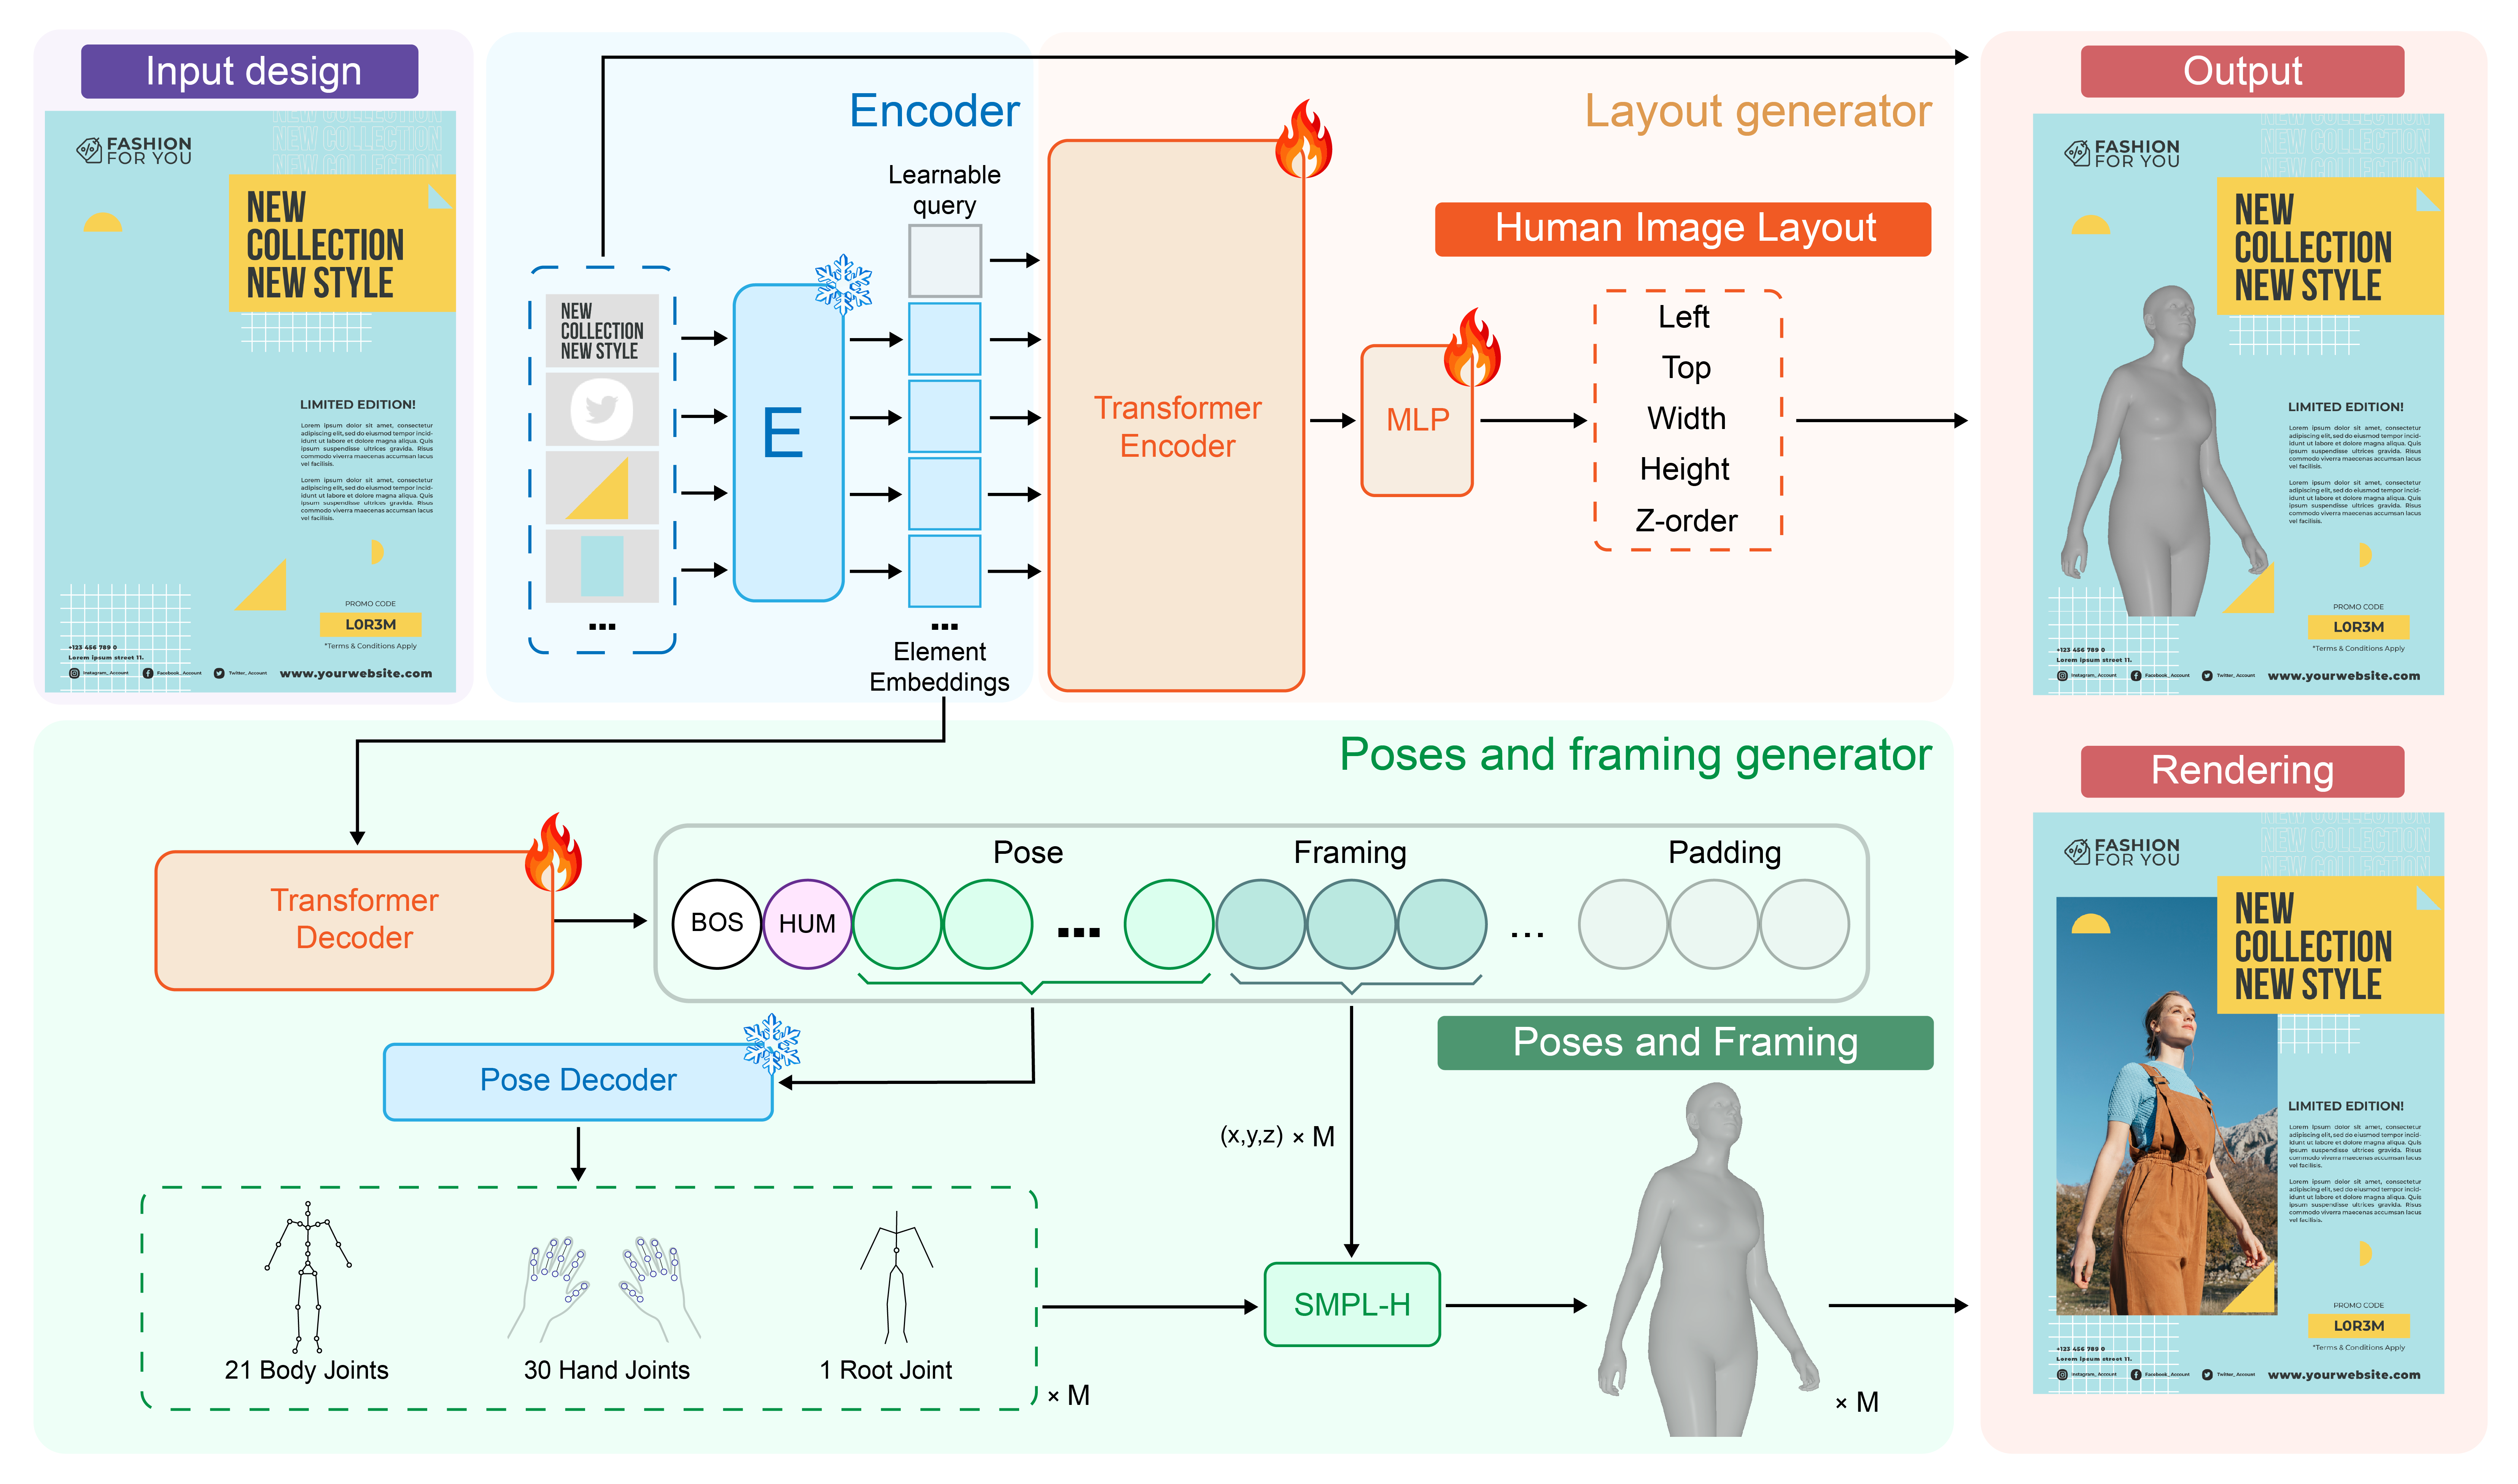
\includegraphics[width=1\linewidth]{figure/fig3_model.png}
  \caption{
  Overview of our model. It takes as input a partial graphic design with a set of multimodal elements (such as images, texts, vector shapes), and generates a complete design with one or several 3D humans added. An encoder is used first used to extract element-wise design embeddings, which are then fed into: a pose and framing generator, a layout generator. The pose and framing generator autoregressively generates pose tokens, which are then decoded into 3D human poses using a pre-trained pose decoder. It also predicts framing tokens that 
  control the composition of the 3D humans in an image. The layout generator takes as input a learnable query and all the element embeddings
  to predict the bounding box parameters and z-order of the human image in the design. With the predicted pose, framing and layout information, the 3D humans are composed into the design, and the 3D human representations can further be rendered as a realistic image.
  }
  \label{fig:model}
\end{figure*}

\subsection{Problem Formulation}
\label{sec:formulation}

Let $\mathcal{D} = \{e_1, e_2, \ldots, e_N\}$ denote an input graphic design consisting of $N$ design elements, where each element $e_i$ is described by a set of attributes: appearance attributes including 
font, color (font color or background color),
opacity; content 
(image or text content); layout attributes
$(c_i, l_i, t_i, w_i, h_i)$ specifying its type $c_i$, 
left position $l_i$, top position $t_i$, width $w_i$, and height $h_i$, respectively. $(l_i, t_i, w_i, h_i)$ are normalized bounding box parameters (with respect to the canvas) in the range $[0, 1]$.
Our objective is to build a model that takes as input a design $\mathcal{D}$, without a human image, and produces the following outputs:
\begin{itemize}
    \item \textbf{Pose}. A sequence of $M$ 3D human poses $P = \{\theta_1, \ldots, \theta_M\}$, where each pose is parameterized by the pose parameters $\theta_i \in \mathbb{R}^{52 \times 3}$ of the SMPL-H model~\cite{smplh},
    which specify 3D angular rotations for 52 joints (21 body joints, 30 hand joints, 1 root joint).
    \item \textbf{Framing}. Framing parameters $F = \{f_1, \ldots, f_M\}$ for $m$ 3D humans. The framing of human $j$ is parameterized by $f_j = (x_j, y_j, z_j)$, which is the global 3D position of the root joint (relative to the camera frame), which determines how the human is framed in the 2D image. 
    \item \textbf{Layout.} A human image layout $L = (l, t, w, h, z)$ that specifies the left position $l$, top position $t$, width $w$, height $h$, and z-order $z$ of the image containing the 3D humans in the design.
\end{itemize}

The generated poses $P$ are rendered into an image using the predicted framing parameters $F$, and placed into the input design according to the predicted image layout $L$, to create a cohesive human-included graphic design. 

\subsection{Our Model}
\label{sec:architecture}

As illustrated in Figure~\ref{fig:model}, our model consists of three main components: 1) a design encoder that extracts design context representations
from the input design, 2) a pose and framing generator that autoregressively generates human pose tokens and framing tokens 
, and 3) a layout generator that predicts the spatial arrangement of the human image. We now describe each component in detail.

\subsubsection{Design Encoder}
The design encoder follows the architecture of FlexDM ~\cite{flexdm}, projecting the elements in the input design into a set of element-wise embeddings.
In particular, for each element, 
the design encoder extracts three types of embeddings from its attributes:
\begin{itemize}
    \item \textit{Appearance embeddings.} We perform discretization on the font, color and opacity, and encode discrete font, color and opacity into separate embeddings 
    through learned embedding layers. 
    When an attribute is missing for an element (e.g., an image element does not have font color), an all-zeros embedding is used.

    \item \textit{Content embeddings.} The visual content is processed through the OpenCLIP~\cite{OpenCLIP} image encoder to obtain an image embedding, while the text content is encoded using OpenCLIP text encoder to produce a text embedding. Then, the image or text embedding is projected into a content embedding through a learned linear project layer.

    \item \textit{Layout embeddings.}
    Each of the four bounding box parameters is discretized. The element type and the discrete bounding box parameters are encoded into layout embeddings through learned embedding layers.
\end{itemize}

The embedding of the element is obtained by adding up its attribute embeddings.
All the element embeddings 
are then processed through a stack of transformer encoder blocks with self-attention layers
to capture inter-element relationships. The encoder finally outputs a sequence of contextualized design element embeddings, 
which we refer to as 
\textit{a design context representation} $\mathbf{C}$ that will be used to condition subsequent generators on information in the input partial design. 

\subsubsection{Pose and Framing Generator}

To generate human poses, we adopt a discrete pose representation inspired by TokenHMR~\cite{tokenhmr}. We first train a Vector Quantized Variational Autoencoder (VQ-VAE) tokenizer specifically for the SMPL-H pose parameters.
The VQ-VAE encoder maps continuous SMPL-H pose parameters $\theta \in \mathbb{R}^{52 \times 3}$ to a discrete token sequence $\mathbf{z}_p = (z_1, z_2, \ldots, z_{400})$, where each token $z_i$ corresponds to a code vector in a learned codebook of size $64$. The VQ-VAE decoder can reconstruct the pose parameters from the tokens: $\hat{\theta} = \mathcal{D}_\text{pose}(\mathbf{z}_p)$.
For framing parameters $f = (x, y, z)$, we discretize each coordinate into 256 bins by applying the K-means clustering on the training set, resulting in a sequence of framing tokens $\mathbf{z}_f = (z_x, z_y, z_z)$.

For $m$ humans, their poses and framing configurations can then be represented as a sequence of discrete tokens:
\begin{equation}
    \mathbf{Z} = (\text{BOS}, \text{HUM}, \mathbf{z}_{p_1}, \mathbf{z}_{f_1}, \ldots, \mathbf{z}_{p_m}, \mathbf{z}_{f_m}, \text{EOS})
\end{equation}
where BOS and EOS are special tokens denoting the start and end of the sequence, and the HUM token is used to signals the start of a human.

Our pose decoder employs an
autoregressive Transformer architecture trained to generate tokens in the sequence $\mathbf{Z}$ iteratively conditioned on the design context representation $\mathbf{C}$ from the design encoder. 
The design context representation is injected into the pose decoder through cross-attention layers. 
The generated pose token sequence $\hat{\mathbf{z}}_p$ is decoded back to the SMPL-H pose parameters using the pre-trained VQ-VAE decoder $\mathcal{D}_\text{pose}$, and the generated framing tokens are converted to continuous framing parameters by taking the bin center values of the tokens.
 

\subsubsection{Layout Generator}

The layout decoder predicts the spatial arrangement of the human image within the design. Our layout decoder utilizes a bidirectional Transformer architecture (with a stack of Transformer encoder blocks), whose inputs include a learnable query (a learnable embedding) and the design context representation $\mathbf{C}$ (a sequence of element embeddings). The query attends to all the element embeddings through the self-attention layers to extract an output query representation (the output embedding of the last Transformer block for the query) that contains necessary information for layout prediction. The output query representation is finally decoded into the layout parameters $(\hat{l}, \hat{t}, \hat{w}, \hat{h}, \hat{z})$ with a  two-layer MLP.

\subsubsection{Human Image Generation and Composition}
Given the generated pose, framing and layout parameters, we can create a human image and compose it into the input design. Specifically, we feed the pose and framing parameters into the SMPL-H model to generate posed 3D human meshes placed in the camera coordinate system, and project the meshes onto an image of size $(W \cdot \hat{w}, H \cdot \hat{h})$, where $(W, H)$ is the canvas size of the input design and $(\hat{w}, \hat{h})$ is the predicted human image size. This results in a transparent human mesh image (where the alpha values of pixels outside the human regions are set to 0), which can be composed into the input design according to the predicted position and z-order $(\hat{l}, \hat{t}, \hat{z})$. To generate a realistic human image, we create a 2D pose map using the 2D projections of the 3D joint positions of the human meshes, and employ LayerDiffuse ~\cite{layerdiffuse} (with SDXL ~\cite{podell2023sdxl} to generate a transparent image conditioned on the pose map, the input design, and a text prompt. The text prompt is generated by Qwen3-VL~\cite{Qwen3-VL} that is queried to describe the human appearance according to the input design. The pose map is incorporated into the SDXL through ControlNet~\cite{controlnet}; the input design is sent into the SDXL through IP-Adapter~\cite{ye2023ipadaptertextcompatibleimage}.

\subsection{Training}
\label{sec:training}

Our model is trained with two task-specific loss functions:

\begin{itemize}
    \item \textit{Pose and framing loss.} The pose and framing generator is trained with a cross-entropy loss for next-token prediction. For a sequence $\mathbf{Z}$ of length $L$. The loss is defined as:
    \begin{equation}
        \mathcal{L}_{\text{PF}} = -\sum_{t=2}^{L} \log p_{\phi}(\mathbf{Z}_t | \mathbf{Z}_{<t}, \mathbf{C}).
    \end{equation}

    \item \textit{Layout loss.} The layout generator is supervised with a combination of a L1 loss and a Generalized IoU (GIoU) loss:
    \begin{equation}
        \mathcal{L}_{\text{L}} = \mathcal{L}_{L1} + \mathcal{L}_{\text{GIoU}}.
    \end{equation}
    $\mathcal{L}_{L_1} = \left| \hat{L} - L \right|$, where $\hat{L}$ and $L$ are the predicted and ground truth human image layout parameters, respectively. $ \mathcal{L}_{\text{GIoU}} = 1 - \text{GIoU}(\hat{B}_{h}, B_{h})$, where $\hat{B}$ and $B$ are the predicted and ground truth bounding boxes of the human image, respectively.

\end{itemize}

During training, we first fine-tune FlexDM on the training component of our dataset (Section \ref{sec:dataset}) and use the obtained corresponding weights to initialize our design encoder. 
Then, we freeze the design encoder weights, and train our model via a three-stage training procedure:
\begin{itemize}
    \item \textit{Stage 1: Pose and framing generator pre-training.} We first train 
    the pose and framing generator using the loss $\mathcal{L}_{\text{PF}}$. This stage allows the pose and framing generator to capture the dependency of human pose and framing on design context. 

    \item \textit{Stage 2: Layout generator pre-training.} We train the layout generator using the loss $\mathcal{L}_{\text{L}}$. This stage enables the layout generator to learn spatial placement of human images based on design context features.

    \item \textit{Stage 3: Joint Fine-tuning.} Finally, we jointly fine-tune the two generators, with a total loss:
    \begin{equation}
        \mathcal{L}_{\text{Total}} = \mathcal{L}_{\text{PF}} + \mathcal{L}_{\text{L}}.
    \end{equation}
    This joint fine-tuning stage allows the two generators to produce the pose, framing and layout that are harmonious with each other.
\end{itemize}

